% ****** Start of file apssamp.tex ******
%
%   This file is part of the APS files in the REVTeX 4 distribution.
%   Version 4.0 of REVTeX, August 2001
%
%   Copyright (c) 2001 The American Physical Society.
%
%   See the REVTeX 4 README file for restrictions and more information.
%
% TeX'ing this file requires that you have AMS-LaTeX 2.0 installed
% as well as the rest of the prerequisites for REVTeX 4.0
%
% See the REVTeX 4 README file
% It also requires running BibTeX. The commands are as follows:
%
%  1)  latex apssamp.tex
%  2)  bibtex apssamp
%  3)  latex apssamp.tex
%  4)  latex apssamp.tex
%
\documentclass[prb,aps,twocolumn,preprintnumbers,amsmath,amssymb]{revtex4}
%\documentclass[preprint,showpacs,preprintnumbers,amsmath,amssymb]{revtex4}

% Some other (several out of many) possibilities
%\documentclass[preprint,aps]{revtex4}
%\documentclass[preprint,aps,draft]{revtex4}
%\documentclass[prb,twocolumn,showpacs,preprintnumbers,amsmath,amssymb]{revtex4}% Physical Review B

\usepackage{graphicx}% Include figure files
\usepackage{dcolumn}% Align table columns on decimal point
\usepackage{bm}% bold math
\usepackage[utf8]{inputenc}
\usepackage{url}
%\nofiles

\begin{document}

\title{Espectros atómicos}% Force line breaks with \\

\author{Alejandro Hernández A.}%
 \email{a.hernandez105@uniandes.edu.co}
\author{Daniel Sánchez M.}%
 \email{d.sanches462@uniandes.edu.co}
\affiliation{%
Departamento de Física\\ Universidad de los Andes, Bogotá, Colombia.\\
}%


\date{3 de septiembre de 2015}% It is always \today, today,
             %  but any date may be explicitly specified

\begin{abstract}
Este informe presenta los datos obtenidos al medir voltaje y corriente para configuraciones solicitadas de circuitos RC y RLC. Para el circuito RC, se determinó el tiempo característico de carga y descarga del condensador, y se otuvieron los siguientes datos: $\tau_{carga} = $ con error porcentual $E\% = \%$ y $\tau_{descarga} = $ con error porcentual $E\% = \%$. Para el circuito RLC, se determinó la frecuencia natural del sistema y el parámetro de resistencia y los datos obtenidos fueron los siguientes: $f_{0} = $ con error porcentual $E\% = \%$ y $\gamma = $ con error porcentual $E\% = \%$. 
\\

%\smallskip
\noindent \textbf{Conceptos clave:} Circuito RC, circuito RLC, oscilador amortiguado.
\end{abstract}
                             
\maketitle

\section{\label{sec:level1}Introducción.}

Las resistencias, condensadores e inductancias son algunos de los elementos electrónicos de dos terminales más usados en diversos dispositivos tegnológicos de la actualidad. Y dado a que la implementación de los circuitos que usan estos elementos es relativamente simple, las características experimentales de estos elementos pueden ser estudiadas rigurosamente, ya sea con corriente directa DC o con corriente alterna AC.\\

En esta práctica nos interesan los circuitos RC y RLC, ambos en serie, cuyas principales características se presentan a continuación.


El circuito a usar se muestra en la figura \ref{fig: RC}

\begin{figure}[h!]
	\centering
	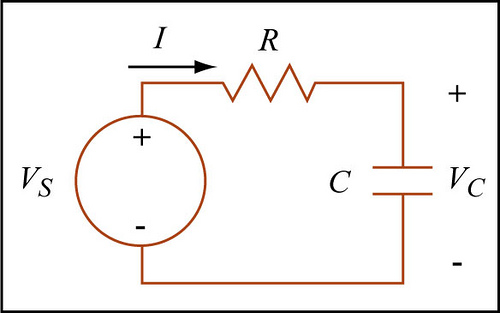
\includegraphics[width=0.4\textwidth]{RC}
	\caption{Circuito RC en serie}
	\label{fig: RC}
\end{figure} 

Para el proceso de carga del condensador, el voltaje a través de la resistencia viene dado por \eqref{VRC}.

\begin{equation}
\label{VRC}
V_{r} = V_{f}e^{-\frac{t}{RC}}
\end{equation}

Donde $V_{f}$ es el voltaje de la fuente (voltaje final del condensador).\\

Para el proceso de descarga el voltaje de la resistencia está dado por \eqref{RC}.

\begin{equation}
\label{RC}
V_{r} = -V_{0}e^{-\frac{t}{RC}}
\end{equation}

Donde $V_{0}$ representa el voltaje inicial del condensador.\\

En las ecuaciones anteriores la constante $\tau = RC$ tiene unidades de tiempo y corresponde al tiempo característico de carga o descarga del condensador de acuerdo a la situación de interés. Para el proceso de carga. Dicha constante es interpretada como el tiempo que tarda en cargarse (o descargarse) el condensador a un $67\%$ de su carga máxima.\\

Ahora bien, el circuito RLC a usar se muestra en la figura \ref{fig: RLC}

\begin{figure}[h!]
	\centering
	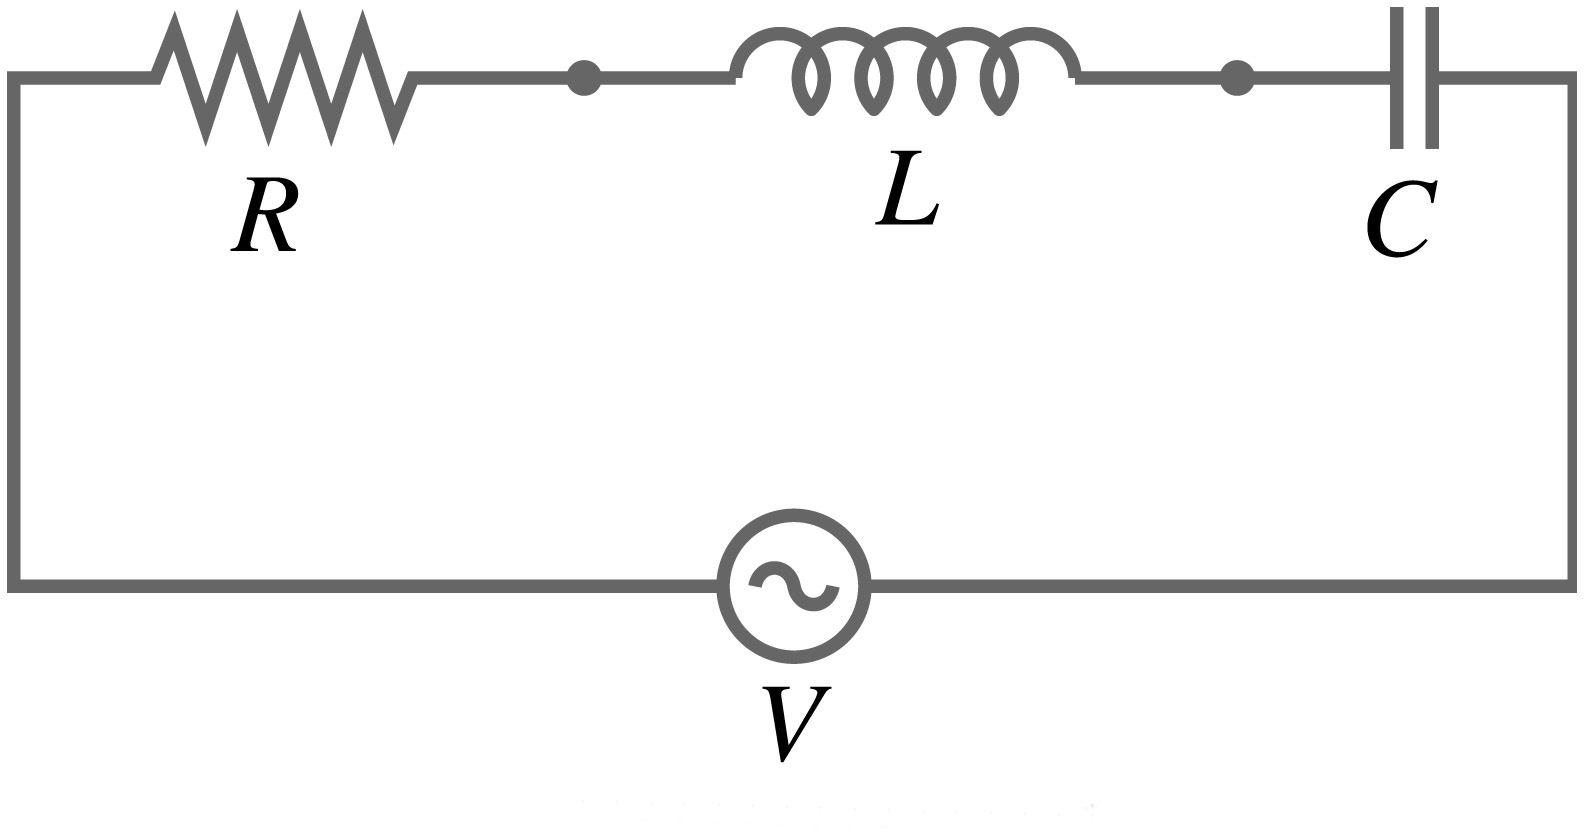
\includegraphics[width=0.4\textwidth]{RLC}
	\caption{Circuito RLC en serie}
	\label{fig: RLC}
\end{figure}

Este circuito es caracterizado por la ecuación \eqref{diff}.

\begin{equation}
\label{diff}
\frac{d^2 q}{d t^2} + \frac{R}{L}\frac{d q}{d t} + \frac{1}{LC}q = V(t)
\end{equation}

Donde $V(t)$ es el voltaje de la fuente, $\gamma = \frac{R}{L}$ es el factor análogo a la fricción en sistemas mecánicos que da cuenta de la disipación de energía en la resistencia, y $\omega_{0}^2 = \frac{1}{LC}$ es la frecuencia natural del sistema.\\

Suponiendo $V = \frac{V_{0}}{L} e^{i\omega t}$, el sistema está forzado y $\omega$ es la frecuencia de forzamiento y los parámetros $\gamma$ y $\omega_{0}$ determinan la resonancia del sistema con respecto al forzamiento  y determinan la existencia o no de soluciones oscilatorias cuando $\omega = 0$. Para dicha dependencia temporal del voltaje, la solución no homogénea de la ecuación \eqref{diff} tiene la forma $q(t) = A(\omega) e^{i \omega t}$, con la amplitud dada por la ecuación \eqref{amplitud}.

\begin{equation}
\label{amplitud}
A(\omega) = \frac{V_{0}}{L}\frac{1}{\sqrt{(\omega^2 - \omega_{0}^2)^2+(\gamma \omega)^2}}
\end{equation}

Y la frecuencia de resonancia (frecuencia en la que la amplitud es máxima) está dada por la ecuación \eqref{resonancia}.

\begin{equation}
\label{resonancia}
\omega_{res} = \sqrt{\omega_{0}^2 - \frac{\gamma^2}{4}}
\end{equation}

De igual manera, el andho de la curva de resonancia está dado por:

\begin{equation}
\label{ancho}
\Delta = \gamma = \frac{R}{L}
\end{equation}

Allende de lo anterior, es preciso hablar de las figuras de Lissajous, ya que serán mencionadas en secciones posteriores de este informe. Las figuras de Lissajous son gráficas de un sistema con ecuaciones paramétricas dadas por:

\begin{equation}
\label{lissa}
\begin{split}
x &= A_{x}\sin(\omega_{x}t + \delta)\\
y &= A_{y}\sin(\omega_{y}t)
\end{split}
\end{equation}

Cabe mencionar que las condición para poder obtener figuras de Lissajous cerradas es que las frecuencias de las dos ondas superpuestas sean conmensurables, es decir, que sean números racionales. La visualización de estas curvas en un osciloscopio permiten verificar experimentalmente las cualidades teóricas de las superposición de en x y y de ondas producidas por un generador de señales.

\section{Montaje experimental}

Los instrumentos usados durante la práctica de laboratorio fueron un osciloscopio, dos generadores de señales, y diversos elementos electrónicos de dos terminales tales como resistencias, inductancias y condensadores.\\

\begin{figure}[h!]
	\centering
	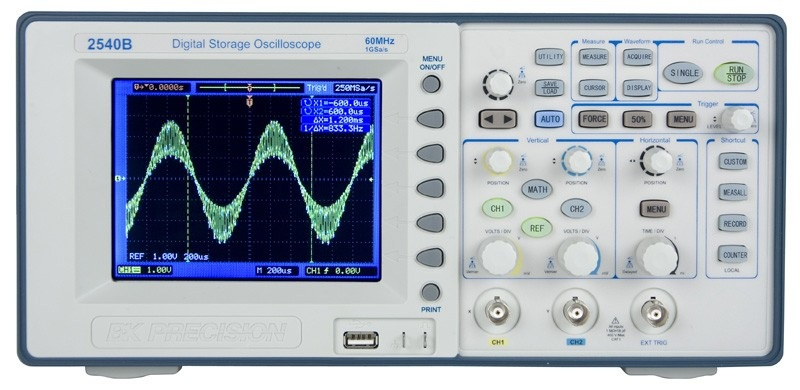
\includegraphics[width=0.4\textwidth]{osci}
	\caption{Osciloscopio usado para tomar de datos.}
	\label{fig: osci}
\end{figure}

\begin{figure}[h!]
	\centering
	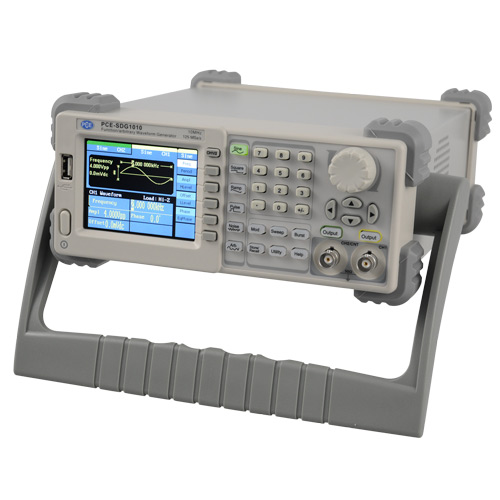
\includegraphics[width=0.4\textwidth,height=0.25\textheight]{generador}
	\caption{Generador de señales usado durante el laboratorio.}
	\label{fig: genr}
\end{figure}

El ocsilador y los generadores de señales se muestran en las figuras \ref{fig: osci} y \ref{fig: genr}.\\

En ensable de los circuitos mostrados en las figuras \ref{fig: RC} y \ref{fig: RLC} se hizo mediante cables proporcionados en el laboratorio, y las mediciones se realizaron con la ayuda de una sonda directamente conectada al osciloscopio que tenía caimanes en sus extremos.\\

En lo que respecta al circuito RC, para realizar las mediciones se usó una onda cuadrada de $5\ Hz$ con una amplitud de $5\ V$, una resistencia de $R = (470 \pm 1)\Omega$ y un condensador de capacitancia $C = (470 \pm 1)\mu F$. Se tomaron datos del voltaje de la resistencia.\\

Por su parte, para el circuito RLC se hicieron dos manipulaciones: en la primera se usó una onda sinusoidal de frecuencia $10\ Hz$ y de amplitud $5\ V$, un condensador de $C = (47 \pm 1)nF$ y una inductancia de $L = (2 \pm 1)mH$. Se tomaron datos del voltaje del condensador y se trató de determinar tanto la curva de resonancia como la frecuencia natural del sistema.\\

Para las figuras de Lissajous se conectaron ambos generadores directamente al osciloscopio, cada uno de generando una onda de amplitud $5\ V$ y mediante el osciloscopio se observó la superposción de estas ondas en el plano $xy$.

\section{Resultados y análisis}

Para el proceso de carga y de descarga del condensador se obtuvieron los datos ilustrados en la figura \ref{fig: carga}




\section{Conclusiones}

\begin{itemize}

	\item La curva de calibración obtenida para el helio, se ajusta bien a las líneas espectrales obervadas para los demás gases, tal y como se muestra en las gráficas de la sección anterior.
	
	\item El valor experimental obtenido para la constante de Rydberg $R_{exp} = (10967597.395 \pm 262058.049)\ m^{-1}$ es muy exacto dado a que el error porcentual de la medida fue de $E\% = 0.055\%$.
		
	\item La observación realizada de las líneas espectrales perimten concluir la validez del modelo de Bohr (o la serie de Balmer) para explicar el espectro de emisión de átomos con un solo electrón, y al tener la hipótesis de cuantización del momento angular, los resultados experimentales obtenidos permiten constatar unad las primeras ideas acerca de cuantización en física.
	
	\item Si bien se obtuvieron buenos resultados, es importante resaltar que tanto la intensidad de las líneas espectrales de los diversos gases, como el grosor de las mismas, da pie para pensar acerca de la realización de medidas con instrumentos de mayor resolución con el fin de obtener mediciones más exactas de la posición de las mismas.
	
\end{itemize}

\begin{thebibliography}{99}
\bibitem{eisberg} R. Eisberg, {\it Quantum Physics of Atoms, Molecules, Solids, Nuclei and Particles}{John Wiley \& Sons, USA, 1985}.\\
\end{thebibliography}

\end{document}
%
% ****** End of file apssamp.tex ******
